% !TeX root = ../paper.tex
% !TeX encoding = UTF-8
% !TeX spellcheck = en_US

\section{Approach}\label{sec:approach}

 %TODO

\begin{itemize}
	\item collect and persist partial results
	\item master worker pattern
	\item at the beginning permutation tree stored only on master (split if it gets too big)
	\item parallelize additional parts of the algorithm (initial pruning)
	\item reaper pattern for clean shutdown
	\item three options for holding the input table:
	\begin{itemize}
		\item \textbf{full replication}
		\item split column wise
		\item split row wise
	\end{itemize}
  \item for the architecture see Figure~\ref{fig:architecture}

  \begin{figure}[p]
    \centering
    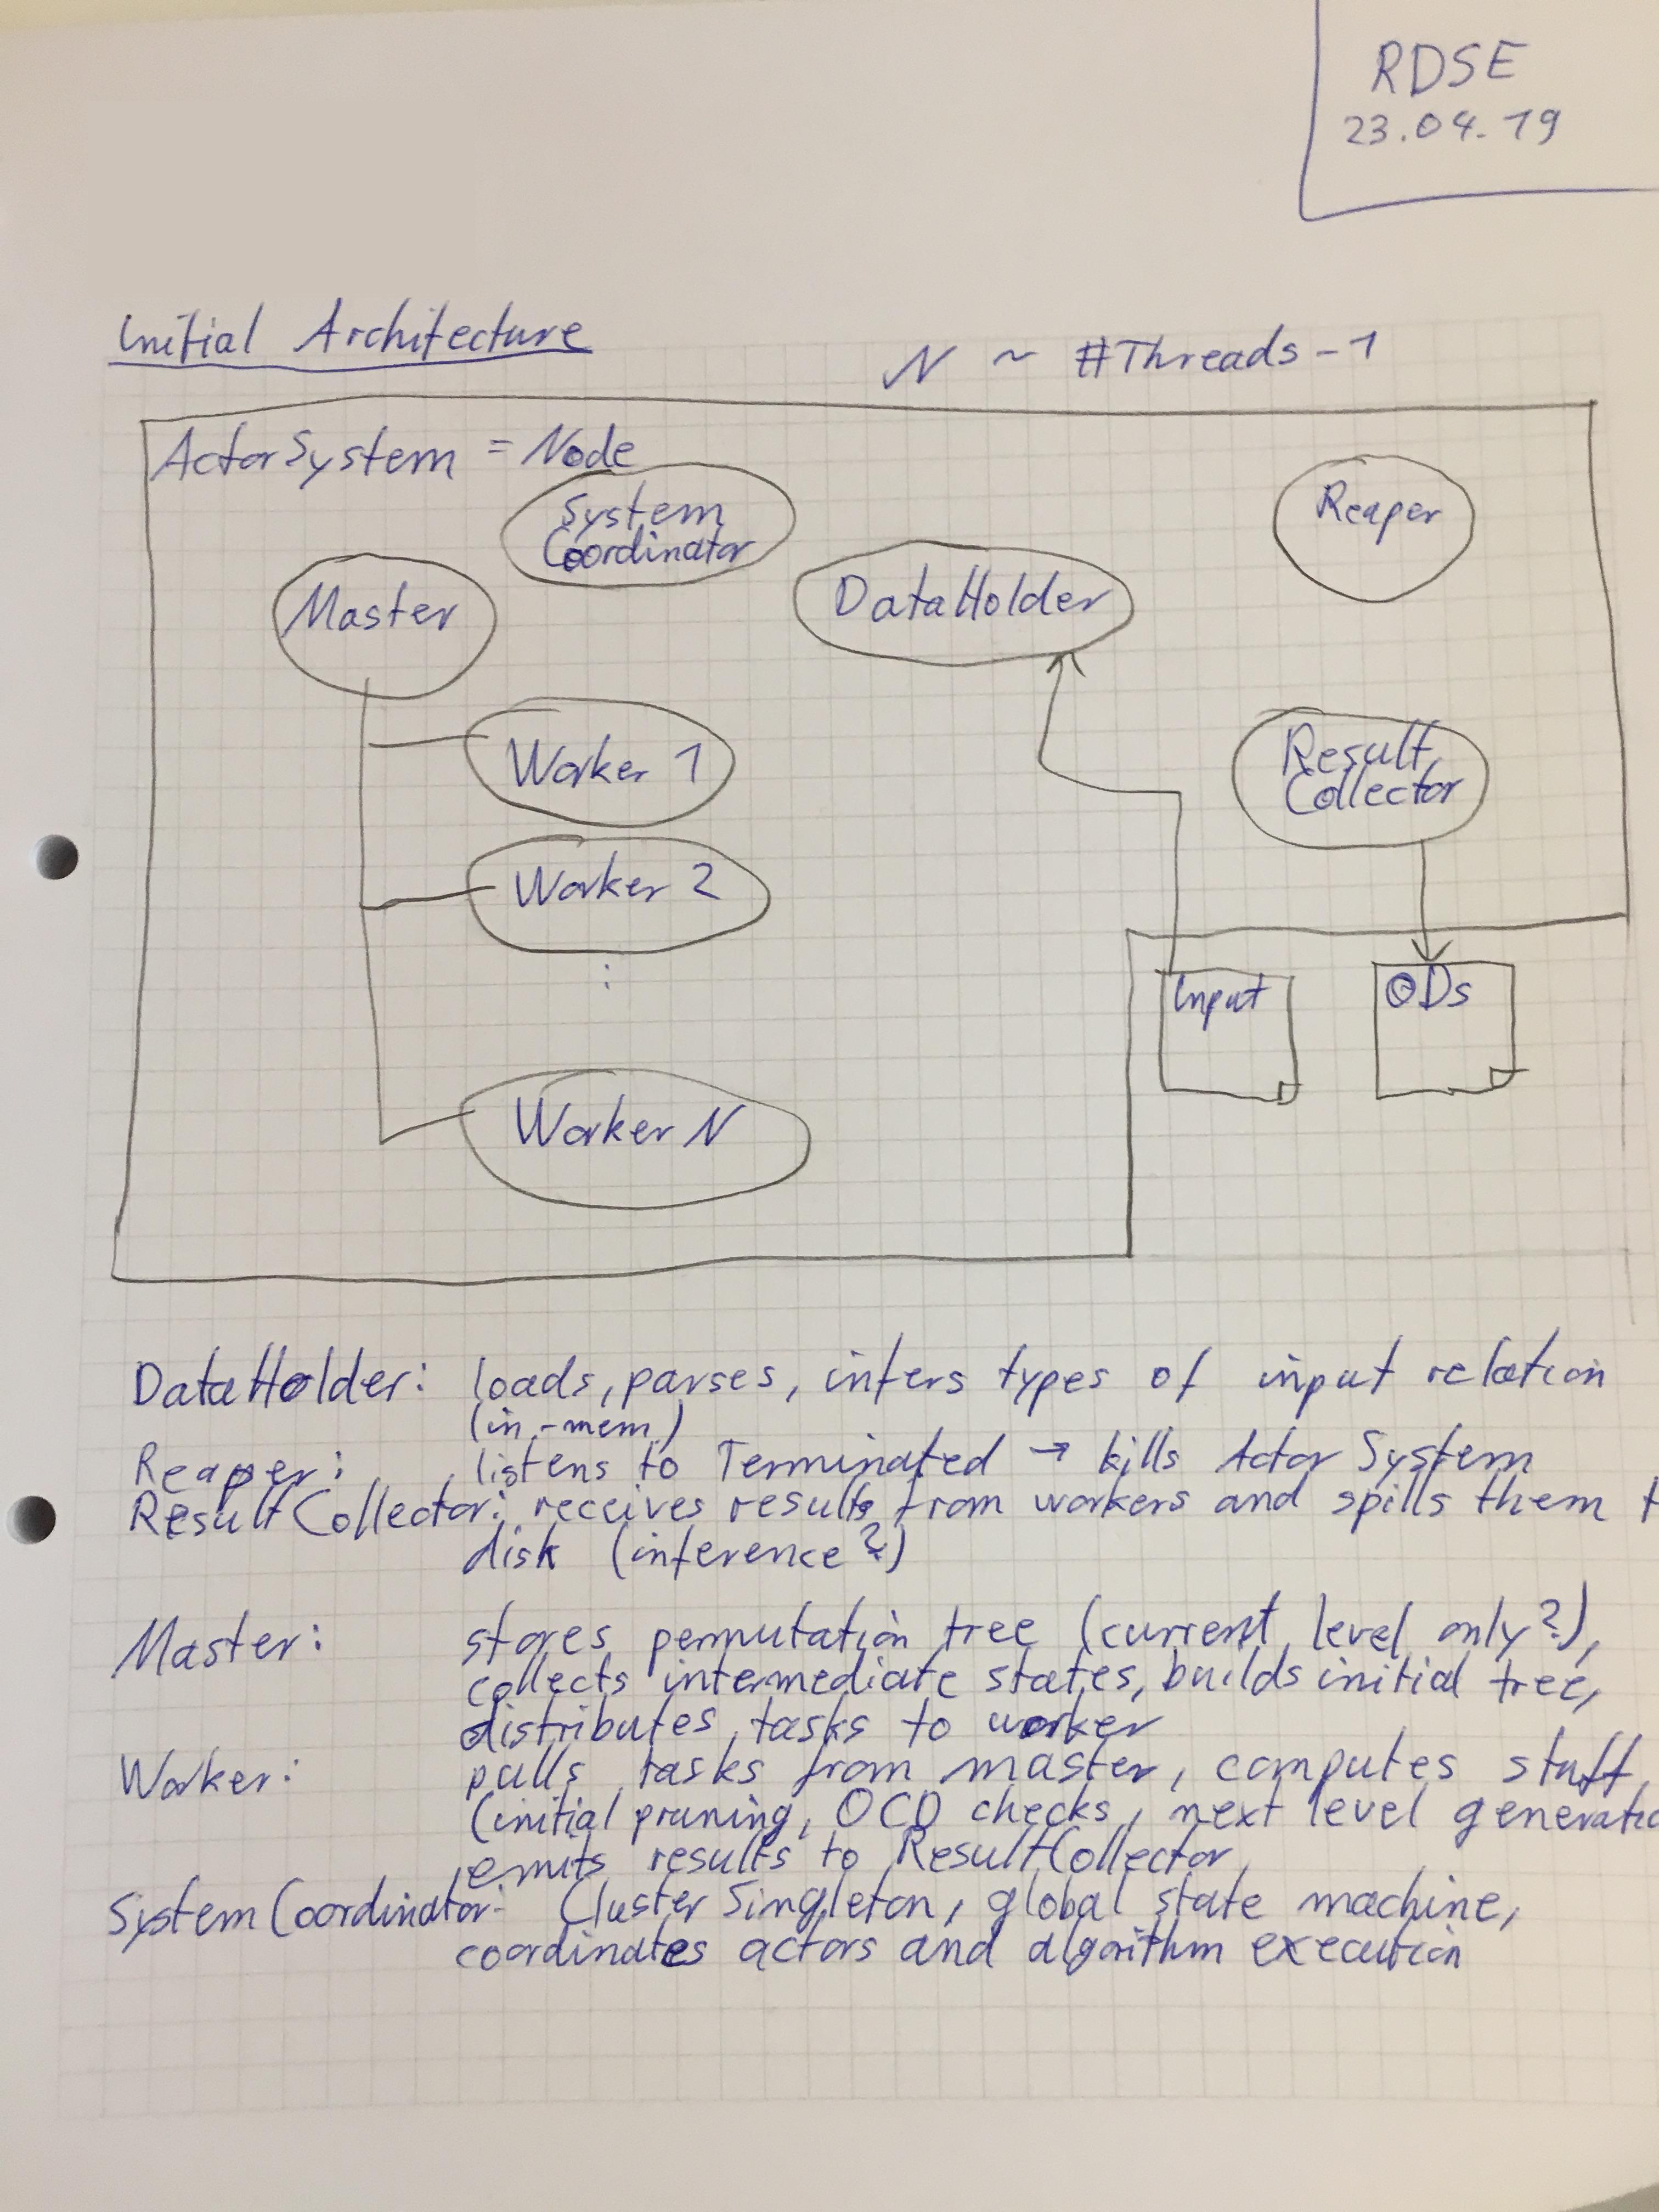
\includegraphics[width=\linewidth]{pictures/actor-architecture.jpg}
    \caption{Actor architecture}
    \label{fig:architecture}
  \end{figure}
	
\end{itemize}